\section{Wired Equivalent Protocol - WEP}


\ac{WEP} is a security protocol, defined in \ac{IEEE}802.11, to secure link-level data throughout wireless transmission. Its message encryption and decryption mechanism was aimed to provide confidentiality, access control and data integrity from data-link layer.

\ac{WEP} mechanism is based on the \ac{RC4} algorithm\cite{mousa2006evaluation} that aims to supply security to \ac{WLAN} equivalent to \ac{LAN}. In general, the \ac{WEP} encryption of a frame includes three steps described in details in \ac{IEEE}802.11 standard \cite{al2006ieee}. The encryption algorithm takes input as a plaintext $M$ and produce the output $C$ and transmit over the network. The three steps of \ac{WEP} would be described as below
\begin{steps}
	\item \ac{WEP} calculate checksum $c(M)$ and concatenate with the original plaintext $M$, we have the message $P = <M, c(M)>$
	\item \ac{WEP} would encrypt the message $P$ achieved in the first step using \ac{RC4}. \ac{RC4} generates a keystream relying on the \ac{IV} $v$ and a key $k$. The keystream is denoted as $RC4(v,k)$. We use \ac{Xor}on the plain text and key stream to get the output $C$ of this step is $C = P \oplus RC4(v,k)$
	\item Concatenate $C$ achieved in step 2 with the \ac{IV} and transmit $<C, v>$ over the network.
\end{steps}

An \ac{AP} would catch the message and decrypt it by using \ac{Xor} operation over the encrypted message with \ac{RC4} key stream.  First, \ac{WEP} would extract message in to $v$ and $C$. After that, a \ac{RC4} keystream would be generated and \ac{Xor} it against $C$ to obtain plaintext $P$:
\begin{center}
	\begin{align}
	P'&= C \oplus RC4(v, k) \\
	&= (P \oplus RC4(v, k)) \oplus RC4(v, k) \\
	&= P
	\end{align}
\end{center}

	
$P$ includes $M$ and checksum $c(M)$. The receiver would split $P$ and check if the checksum is matched or not. The whole protocol of \ac{WEP} is described in \autoref{fig:wep}
\begin{figure}
	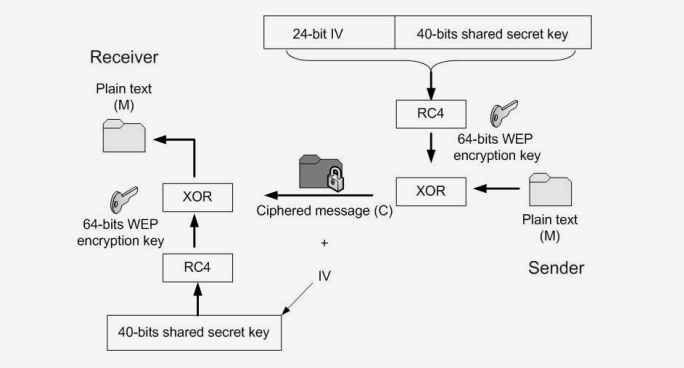
\includegraphics[scale=0.35]{images/wep.png}
	\caption{The WEP protocol \cite{al2006ieee}}
	\label{fig:wep}
\end{figure}

However, this scheme would cause a serious problem if two cipher texts use the same \ac{RC4} key stream. Due to the \ac{Xor} operation properties, the \ac{Xor} operation over two ciphertext using the same key stream will result as the \ac{Xor} operation over two corresponding plaintexts:

\begin{align}
	C_1 &= P_1 \oplus RC4(v,k)\\
	C_2 &= P_2 \oplus RC4(v,k) \\
	C_1 \oplus C_2 &= (P_1 \oplus RC4(v,k)) \oplus (P_2 \oplus RC4(v,k))\\
	C_1 \oplus C_2 &= P_1 \oplus P_2
\end{align}

The above peril property of \ac{RC4} might incapacitate most of the security goals in \ac{WLAN} as the attacker might know $P_1$ or $P_2$ and do the \ac{Xor} operation again to get the original plaintext of others. This means that any adversary who know a plaintext can use it to decrypt others. In case that an adversary obtains these two conditions:
\begin{itemize}
	\item Ciphertexts that use the same keystreams.
	\item The availability of several plaintexts.
\end{itemize}
he or she would negate all the efforts of \ac{WEP} to provide confidentiality  outrageously. Unfortunately, both of the above conditions could absolutely be achieved by skillful and patient attackers.

\citeauthor{borisov2001intercepting} in \cite{borisov2001intercepting} discuss